%\documentclass[handout]{beamer}
\documentclass{beamer}

% Customize slide appearance
\mode<presentation>
{
  \usetheme{default}
  \setbeamercovered{transparent}
}

\usepackage[english]{babel}
\usepackage{times}
\usepackage{threeparttable}
\usepackage{tabularx}
\usepackage{booktabs}
\usepackage{pgfpages}

\definecolor{darkblue}{rgb}{0.1,0,0.55} \definecolor{darkgreen}{rgb}{0,0.7,0}
\definecolor{important}{rgb}{0.9,0.1,0.1} %
\definecolor{hidden}{rgb}{0.8,0.8,0.8}
\definecolor{darkgreen}{rgb}{0,0.7,0}

%\pgfpagesuselayout{4 on 1}



\AtBeginSection[]
{
  \begin{frame}
  \frametitle{Outline}
  \large{\tableofcontents[currentsection,hideothersubsections]}
  \end{frame}
}


%\usepackage{amstext}

\begin{document}

\begin{frame}

\bigskip

\center{{\Large \textcolor{darkblue}{Seeing is Believing: \\ The Effect of Television on the Identity and Lives of Hispanic People}} \medskip}

\bigskip


\center{\textbf{Andrew Kao} \\ \textit{University of Chicago}}

\bigskip \bigskip

\center{February 2020}

\end{frame}

\begin{frame}
\frametitle{Motivation}


\begin{itemize}
\item Large literature on how TV affects behavior {\footnotesize(Yanigazawa-Drott 2014; DellaVigna \& al. 2007;  Ferrara \&\ al., 2012)}
\item 50\% of Hispanics watch satellite or broadcast Spanish Language TV
\item Complicated time for largest ethnic minority in the US
\item Prior efforts to study Hispanic interaction with media focused on politics {\footnotesize(Waldfogel \& al. 2009; Trujillo \& al. 2012)}
\end{itemize}

This paper:\\
\textbf{\,\,\,\, (1) How does Hispanic behavior change in firms and schools?}\\
\textbf{\,\,\,\,  (2) How is identity affected?}

\begin{itemize}
\item Identification: follow Velez \& Newman (2019) and construct spatial RD arising from FCC TV signal regulation
\end{itemize}




\end{frame}


\begin{frame}
\frametitle{Main Findings - Firms}

\centering
        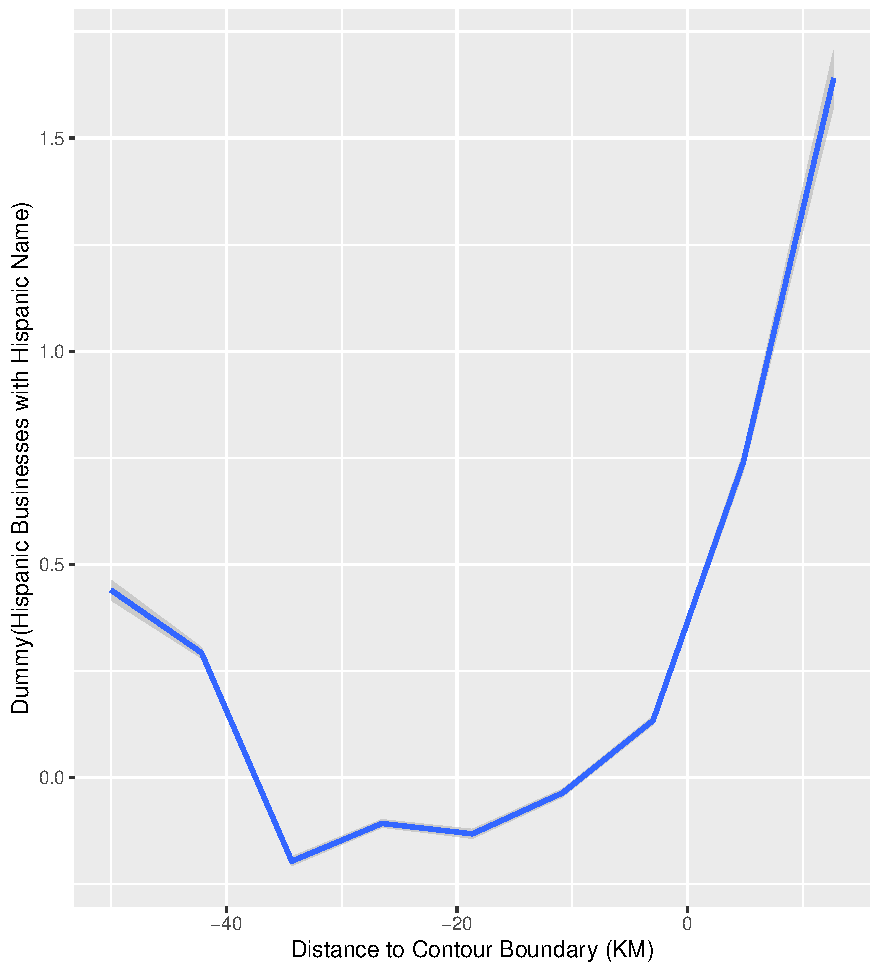
\includegraphics[width=0.65\textwidth]{../../analysis/Output/graphs/hispanicbusnname.pdf}\\
\end{frame}

\begin{frame}
\frametitle{Main Findings - Schools}
\centering
        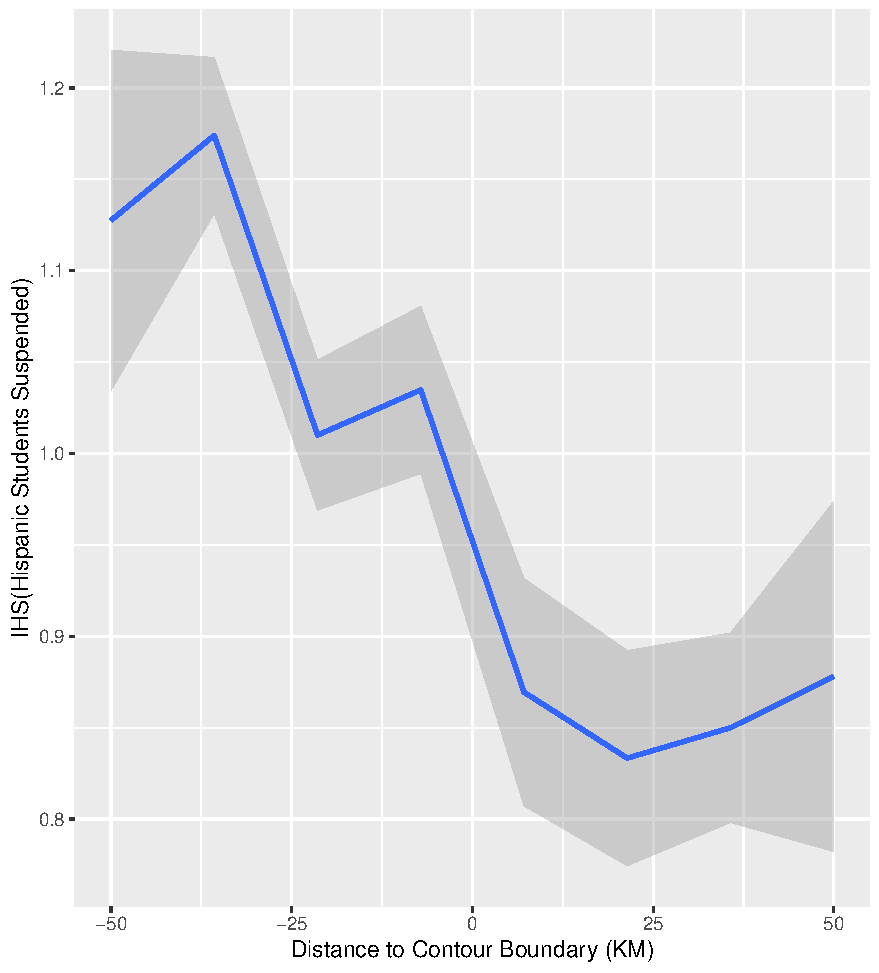
\includegraphics[width=0.65\textwidth]{../../analysis/Output/graphs/hispanicsuspensions.pdf}\\
\end{frame}

\begin{frame}
\frametitle{Main Findings - Campaign Contributions}
\centering
        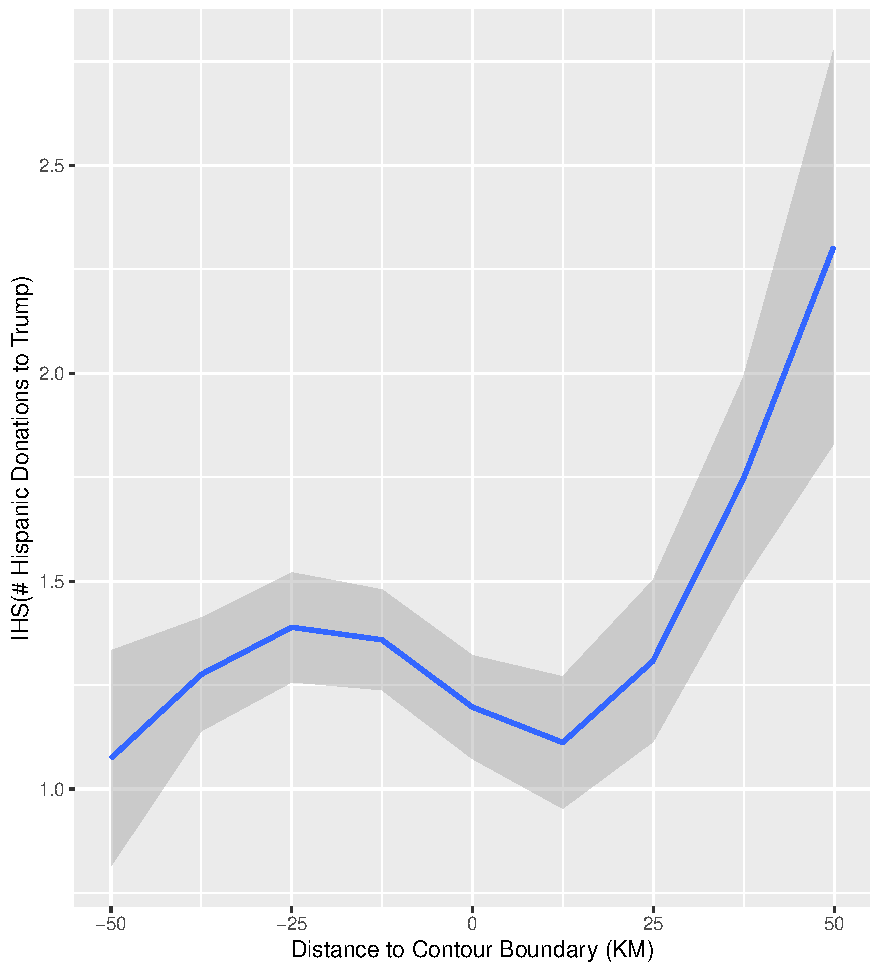
\includegraphics[width=0.65\textwidth]{../../analysis/Output/graphs/hispanictrump.pdf}\\
\end{frame}



%\begin{enumerate}
%\item<1-> 
%White Americans living alongside Arab immigrants
%and Arab-Americans become more positively inclined towards Arabs as the result of this exposure. 
%\item<2-> Long-term exposure to descendants from a given foreign origin country prompts white Americans to donate more generously to that country in times of need (disasters, droughts, epidemics...).
%\item<3-> This positive effect of exposure 
%\item[-]<3->is statistically significant along the entire political spectrum -- operates even in very conservative counties. 
%\item[-]<3-> is specific to ethnicities that white Americans are exposed to and is statistically significant even after controlling for overall racism or general attitudes to foreigners.
%\item[-]<3-> is stronger for genetically more distant origin countries.
%\end{enumerate}
%
\begin{frame}
\frametitle{Contribution}
\begin{itemize}

\item Existing work on Hispanic communities often geographically constrained \& media studies only concerned with effect on politics  {\footnotesize (Velez \& Newman (2019); Trujillo \& al. 2012)}. 
\item[$\rightarrow $] \textcolor{darkblue}{Identify causal effect on larger scale and with more granularity (geocoded microdata)}

\item[$\rightarrow $] \textcolor{darkblue}{Provide a first look at how media affects business and schooling outcomes for Hispanics}

\item New research on how identity is constructed and strengthened {\footnotesize (Atkin \& al. 2019; Bazzi \& al. 2019)}

\item[$\rightarrow $] \textcolor{darkblue}{Supply a revealed preference link to how identity can be bolstered by TV}

\end{itemize}

\end{frame}


\begin{frame}
\frametitle{Empirical Strategy}
\begin{itemize}

\item OET Bulletin No. 69 --- protect TV stations in (50,90) coverage contour areas
\begin{itemize}
\item Mechanical formula based on geographic/technical factors (not political/economic)
\item Fairly large boundaries that typically cut through small towns/suburbs
\item Purchase/constructed antennas prior to 1977
\end{itemize}
\item Spanish Language TV: Isolate effect on Hispanic communities
\item Both RD and instrument with distance
\begin{itemize}
\item Keep observations within 100 KM of boundary for comparability
\item Focus on the RD, dummy for whether observation falls inside contour
\end{itemize}

\end{itemize}

\end{frame}

\begin{frame}
\frametitle{Coverage Map for TV Station WUVC-DT}
\centering
        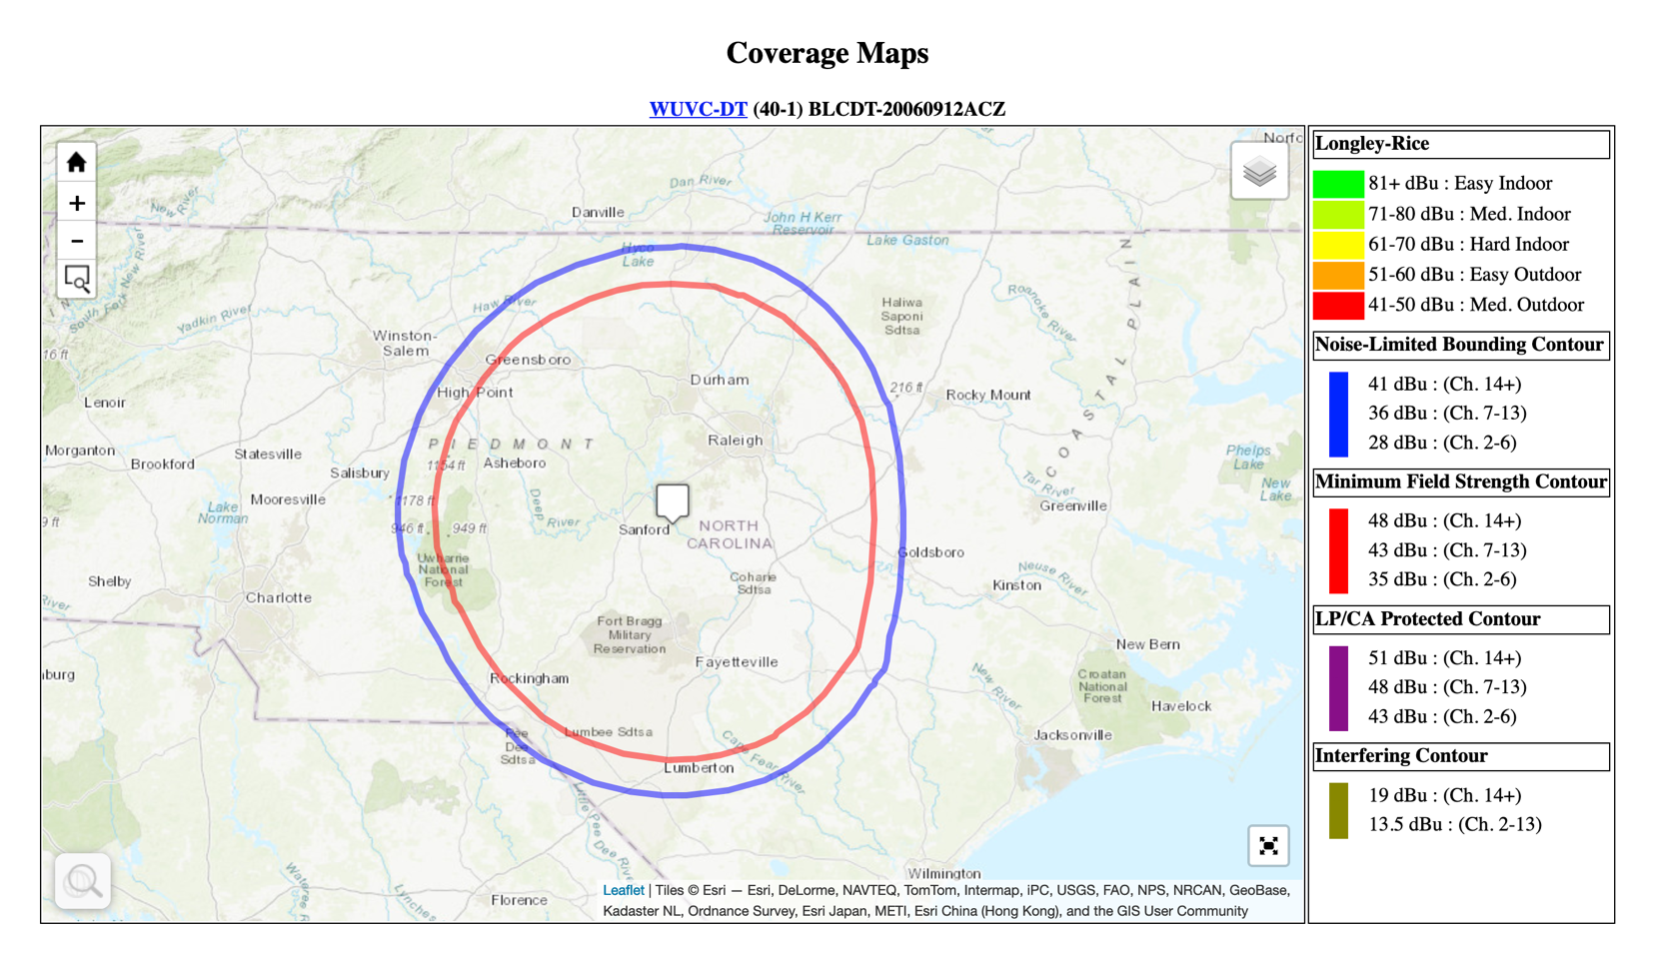
\includegraphics[width=1\textwidth]{../../analysis/Output/img/ContourExample.png}\\
\end{frame}

\begin{frame}
\frametitle{Specifications}

\textbf{Main Model:}
\[ Y_i^{} = \beta_0 + \beta \mathbb{I}[InsideContour_i] \times Distance_i + \gamma X_i + \epsilon_i \, \, \, \, \, \, \, \epsilon \stackrel{iid}{\sim}   N(0,\sigma_i^{2})\]

\textbf{Spatial Autogressive:}
\[ Y = \beta_0 + \rho W Y + \beta \mathbb{I}[InsideContour] \times Distance + \gamma X + \epsilon \]

\textbf{Spatial Error:}
\[ Y = \beta_0 + \beta \mathbb{I}[InsideContour] \times Distance + \gamma X + \epsilon \]
\[\epsilon = \lambda W \epsilon + \nu\]

where $W$ is a 4 nearest neighbor/rook spatial weights matrix

\end{frame}

\begin{frame}
\frametitle{Data - General}

\begin{itemize}
\item Instrument:
\begin{itemize}
\item Identify 100 Spanish Language TV stations across the US from TMS
\item Station contours and other station data from the FCC (use data from 2015 for consistency with outcomes)
\end{itemize}
\item Geocoding:
\begin{itemize}
\item ArcGIS: 99\%+ successfully geocoded, but data limit (schools and small number of campaign contributions)
\item US Census Geocoder: 80\% successfully geocoded (firms and campaign contributions)
\end{itemize}
\item Demographic and migration information at county level from ACS
\end{itemize}

\end{frame}

\begin{frame}
\frametitle{Selection? Migration?}
\begin{center}
        \scalebox{.5}{
	\begin{threeparttable}
			\begin{tabular}{lcccccccccc}
				\hline\hline\addlinespace
				& \multicolumn{3}{c}{IHS(\# Hispanic Migrants)} \\
				\cline{2-4} 
				Panel A: Origin County Inside Contour&  (1) & (2) & (3) \\
                                \hline\addlinespace
Dummy: Destination Outside TV Contour & $-$0.387$^{***}$ & $-$0.286$^{***}$ & $-$0.280$^{***}$ \\ 
  & (0.048) & (0.044) & (0.044) \\ 
 TV Dummy $\times$ Distance to Origin & $-$0.003$^{**}$ & $-$0.004$^{***}$ & $-$0.004$^{***}$ \\ 
  & (0.001) & (0.001) & (0.001) \\ 
 TV Dummy $\times$ Distance to Destination & 0.001 & $-$0.002$^{*}$ & $-$0.002 \\ 
  & (0.001) & (0.001) & (0.001) \\ 
 Distance from Contour to Origin (KM) & 0.001 & 0.003$^{*}$ & 0.003 \\ 
  & (0.002) & (0.002) & (0.002) \\ 
 Distance from Contour to Destination (KM) & $-$0.001 & 0.002 & 0.002 \\ 
  & (0.001) & (0.001) & (0.001) \\ 
Observations & 8,479 & 8,479 & 8,479 \\ 
\hline\addlinespace
Panel B: Origin County Outside Contour & & & \\ 
\hline\addlinespace
 Dummy: Destination Inside TV Contour & $-$0.078 & $-$0.123 & $-$0.120 \\ 
  & (0.108) & (0.096) & (0.096) \\ 
 TV Dummy $\times$ Distance to Origin & $-$0.003$^{*}$ & $-$0.004$^{***}$ & $-$0.004$^{***}$ \\ 
  & (0.002) & (0.001) & (0.001) \\ 
 TV Dummy $\times$ Distance to Destination & $-$0.004$^{***}$ & $-$0.002 & $-$0.002 \\ 
  & (0.001) & (0.001) & (0.001) \\ 
 Distance from Contour to Origin (KM) & $-$0.0003 & 0.001 & 0.001 \\ 
  & (0.001) & (0.001) & (0.001) \\ 
 Distance from Contour to Destination (KM) & $-$0.001$^{***}$ & $-$0.001$^{***}$ & $-$0.001$^{***}$ \\ 
  & (0.0002) & (0.0003) & (0.0003) \\ 
Observations & 4,062 & 4,062 & 4,062 \\         
\hline\addlinespace
                                Log(Population) & Yes & Yes  & Yes\\
                                County \% Hispanic & No & Yes & Yes\\
                                Log(Income) & No & No & Yes\\
				\addlinespace\hline\hline
			\end{tabular}
			\begin{tablenotes}[flushleft]
				\item \textit{Notes:} County-county data with origin F.E. 
			\end{tablenotes}
		\end{threeparttable}

        }
\end{center}
\end{frame}

\begin{frame}
\frametitle{Firms}

\begin{itemize}
\item Data from Florida's Division of Corporations
\begin{itemize}
\item Why Florida? 23\% Hispanic (8\% US total), 11 SLTV stations (11\% total) and open data
\item 146,032 firms successfully geocoded
\item Aggregate data into $2\times 2$ KM$^2$ squares
\end{itemize}
\item Firm Owner Name Classification
\begin{itemize}
\item `ethnicolr' --- a LSTM model trained with TensorFlow on Florida voter registration data
\item Validation $>85\%$ accurate, $23.5\%$ firm owners are Hispanic
\end{itemize}
\item Firm Name Classification
\begin{itemize}
\item Keyword matching on (1) references to Latin American countries, (2) top 50 most common Spanish words not in English, and optionally (3) references to common Hispanic foods
\item 1\% (1.1\% with food) of firms match this criteria
\end{itemize}
\end{itemize}
% SUMMARY STATS BUTTON
\end{frame}


%
%
%\begin{frame}
%\frametitle{Charitable Donations to Foreign Countries}
%
%\begin{itemize}
%\item Data from 2 large charitable organizations (no clearance to divulge their names yet):
%\begin{itemize}
%\item \texttt{Charity 1}.
%\item \texttt{Charity 2}.
%\end{itemize}
%\item Donations to foreign causes only (countries in distress).
%\item Data on:
%\begin{itemize}
%\item Location of donor (county).
%\item Name of donor (more later).
%\item Date of donation.
%\item Country targeted.
%\item Amount donated (\texttt{Charity 2} only).
%\end{itemize}
%\item \texttt{Charity 1}: 60,000 donations from 3,141 counties to 31 countries, 2005 - 2018.
%\item \texttt{Charity 2}: 690,000 donations from 3,141 counties to125 countries, 2011 - 2018.
%\end{itemize}
%
%\end{frame}
%
%
%\begin{frame}
%\frametitle{Charitable Donations: Disasters}
%
%\begin{itemize}
%\item Definition of a ``disaster'':
%\begin{itemize}
%\item At least 2 consecutive months,
%\item with at least 5 donations,
%\item going to the same country.
%\end{itemize}
%\item Top 5 disasters (number of donations, \texttt{Charity 1}):
%\begin{itemize}
%\item Nepal Earthquake 2015 (10,126)
%\item Haiti Earthquake 2010 (9,855)
%\item Indonesia Tsunami 2004 (8,331)
%\item Japan Earthquake/Tsunami 2011 (8,232)
%\item Sudan Darfur 2003 (3,779)
%\end{itemize}
%\item Top 5 disasters, Arab countries (number of donations, \texttt{Charity 1}):
%\begin{itemize}
%\item Sudan Darfur 2003 (3,779)
%\item Yemen Civil War 2015 (2,022)
%\item Somalia Famine 2012 (2,007)
%\item Syria Civil War 2011 (812)
%\item Libya Civil War 2011 (234)
%\end{itemize}
%\end{itemize}
%
%\end{frame}
%
%
%\begin{frame}
%\frametitle{Donors' Name Matching (1/2)}
%
%\begin{itemize}
%\item Partnership with consulting firm \texttt{NAMSOR}.
%\item Match first \& last names with most likely national origin:
%\begin{itemize}
%\item Likeliest origin for ``Donald TRUMP'': Great Britain.
%\item Likeliest origin for ``Barack OBAMA'': Kenya.
%\end{itemize}
%\item Systematically remove donors of non-European ancestry:
%\begin{itemize}
%\item E.g. Haitian American donating to Haiti Earthquake Relief.
%\end{itemize}
%\item Protocol to ensure donors' privacy:
%\begin{itemize}
%\item We never see any name.
%\item \texttt{NAMSOR} sees only names.
%\item \texttt{NAMSOR} deletes all data after disambiguation.
%\item Charitable organization does matching in-house.
%\item All data aggregated into counties $\times$ countries.
%\end{itemize}
%\end{itemize}
%
%\end{frame}
%
%
%
%
%\begin{frame}
%\frametitle{County-level Measure of Exposure}
%
%
%
%\begin{itemize}
%\item[$\bullet$] \texttt{IPUMS} datasets from the \texttt{US Census of population}.
%\item[$\bullet$] Censuses: 1880-2010
%\item[$\bullet$] Variables:
%
%\begin{itemize}
%\item[-] Current location (US county) [all];
%\item[-] Ancestry [2010];
%\item[-] Birthplace [all];
%\item[-] Year of immigration [1900-];
%\item[-] Birthplace of mother and father [1880].
%\end{itemize}
%\end{itemize}
%\medskip
%
%\textbf{Measure of long-term exposure}
%\begin{description}
%
%\item[$A^{2010}_{o,d} =$] \# of individuals in $d$ with ancestry in $o$.
%\end{description}
%
%\medskip
%
%\textbf{For instrumentation also construct}
%\begin{description}
%\item[$I_{o,d}^t = $] \# individuals in US county $d$ born in foreign country $o$ who immigrated between $t$ and $t-1$.
%
%\end{description}
%
%\end{frame}
%
%%%%%%%%%%%%%%%%%%%%%%%%
%% 3 slides on identification (intuition)
%%%%%%%%%%%%%%%%%%%%%%%%
%
%\section{Estimating the causal effect of exposure}
%
%\begin{frame}
%\frametitle{Empirical Strategy}
%\begin{itemize}
%\item Estimate effect of exposure ($A^{2000}_{o,d}$) on attitudes and actions ($y^{t}_{o,d}$) of White residents of county \(d\) towards minorities or foreigners from country \(o\).
%$$y^{t}_{o,d}=\delta_t+\delta_o+
%\delta_d+\beta A^{2000}_{o,d}+X_{o,d}'\gamma+\varepsilon_{o,d} $$
%\item[1.] Use a destination FE or parametric controls for general attitudes towards minorities and political leanings in \(d\).
%\item[2.] Isolate quasi-random variation in \(A^{2000}_{o,d}\) from historical migrations {\footnotesize(Burchardi, Chaney, and Hassan, 2018)}.   
%\end{itemize}
%\end{frame}
%
%
%\begin{frame}
%\frametitle{Instrument for Ancestry}
%
%\begin{equation*}A^{2010}_{o,d}=\delta_{o}+\delta_{d}+X_{o,d}'\xi+\sum_{s=1880}^{t}\beta^s_{r(d)} \tilde{I}_{o,-r(d)}^s\frac{I_{-c(o),d}^s}{I_{-c(o)}^s}+u_{o,d}^t\label{eq:A}\end{equation*}
%
%\begin{itemize}[<+->]
%\item Predict today's ancestry using interaction of:
%\begin{itemize}
%\item[PUSH.]<.-> Staggered arrival of migrants from different origins.
%\item[PULL.]<.-> Variation over time in the attractiveness of different US destinations for the average migrant arriving at that time.
%\end{itemize}
%\item<+-> To avoid confounding factors, leave-out big chunks of migrants (regions and continents: $-r(d)$ and $-c(o)$ terms).
%\item<+-> \textcolor{darkblue}{Example:} Large community with Mexican ancestry in Detroit explained by:
%\begin{itemize}
%\item[PUSH.]<.-> Large migrations from Mexico to the US in 1910-20 (Mexican Revolution).
%\item[PULL.]<.-> Detroit attracts migrants from all origins in 1910-20 (automobile boom).
%\end{itemize}
%\end{itemize}
%\end{frame}
%
%
%
%
%
%
%%%%%%%%%%%%%%%%%%%%%%%%
%%
%%\begin{frame}
%%\frametitle{Empirical Strategy}
%%\begin{itemize}
%%\item Estimate effect of exposure on attitudes and actions of White residents of county \(d\) towards minorities or foreigners from country \(o\).
%%$$y^{t}_{o,d}=\delta_t+\delta_o+
%%\delta_d+\beta A^{2000}_{o,d}+X_{o,d}'\gamma+\varepsilon_{o,d} $$
%%\item[1.] Use a destination FE or parametric controls for general attitudes towards minorities and political leanings in \(d\).
%%\item[2.] Isolate quasi-random variation in \(A^{2000}_{o,d}\) that is orthogonal to all \(o-d\)  specific factors; arises solely from interaction of
%%
%%\smallskip
%%
%%(1) the staggered arrival of migrants from different origins 
%%\smallskip
%%
%%\centering{ -and-} 
%%\flushleft
%%(2) variation over time in the attractiveness of different US destinations for the average migrant arriving at the time {\footnotesize (Burchardi, Chaney, and Hassan, 2018)}.   
%%\end{itemize}
%%\end{frame}
%
%
%
%\section{The Effect of Exposure on Attitudes Towards Arabs}
%
%\begin{frame}
%\frametitle{Effect of Arab Ancestry Attitudes Toward Arab-Muslims}
%\label{iat regs}
%%FIXMEAT: Report Table 2 as follows:
%%Column 1 of Panel B
%%followed by columns 1,3,4,5  of Panel A
%
%\begin{center}
%        \scalebox{.7}{
%                \begin{threeparttable}
%                        \begin{tabular}{lcccccccccc}
%                                \hline\hline\addlinespace
%                                Panel A: & \multicolumn{5}{c}{\textit{Avg Score on Arab-Muslim IAT}} \\
%                                \cmidrule{2-6} & (1) & (2) & (3) & (4) & (5) \\
%                                & OLS & IV & IV & IV &IV \\
%                                \hline\addlinespace
%%                                \input{../Input/IAT_present_5_IV.tex} \addlinespace\hline
%                                Forced Response & No & No & Yes & Yes  & Yes  \\
%                                Demographic Controls & No & No & No & Yes & Yes  \\
%                                \addlinespace\hline\hline
%                        \end{tabular}
%                        \begin{tablenotes}[flushleft]
%                                \item \textit{Notes:} Higher score means a more positive attitude towards Arab-Muslims. Demographic controls include 2010 population density, share of 1970 prime-age population with high school education, and share of 1970 prime-age population with college education. Standard errors are robust.
%                        \end{tablenotes}
%                \end{threeparttable}
%        }
%\end{center}
% \hyperlink{appendix: individual}{\beamergotobutton{Individual Level Regressions}}
%\end{frame}
%
%
%\begin{frame}
%
%
%
%\begin{frame}
%\frametitle{Remaining challenges}
%\begin{itemize}
%\item[A.] 
% A common unobserved
%characteristic of destinations in two different census
%regions, correlated with attitudes today, may still have
%disproportionately caused large groups of migrants from
%two origins on two different continents to simultaneously and repeatedly
%migrate to the same destinations across census regions.
%\item[-] Very hard to come up with examples.
%\item[-] Show same results with differently constructed instruments to exclude this possibility.
%\item[B.] Heterogeneous and directed white flight: different types of white people prefer Somalis to Haitians, and vice versa, and therefore endogenously migrate to counties with their preferred minorities.  
%\item[-] Show results with and without most ``hated'' minorities.
%\end{itemize}
%
%
%\end{frame}
%
%
%\begin{frame}
%\frametitle{Alternative Instruments}
%%FIXMEAK Paste results with different instruments here. Vertical table as in Table 5 of EMIT. Line 1 has standard specification for comparison.
%
%\begin{center}
%        \scalebox{.6}{
%               \begin{threeparttable}
%                        \begin{tabular}{l@{\extracolsep{4pt}}cccc}
%\hline\hline   & Charity 1 & & Charity 2 & \\
%                                                                         \hline\addlinespace Panel A: Variations of leave-out categories   & \multicolumn{1}{c}{IHS(\#\ Donations)} & $F$-Stat & IHS(\#\ Donations) & $F$-Stat \\
%                                \hline
%  \\
%                                Standard Specification  &     0.076** & 54.0 & 0.031** & 212.4 \\
%                                    &     (0.032) & & (0.016)  \\
%                                Europe Only Pull Factor &     0.081** & 46.4 & 0.037** & 61.0 \\
%                                &     (0.031) & & (0.017) \\   
%                                Excluding Origins with Correlated Migration Flows &     0.086* & 36.8 & 0.080** & 122.8\\
%                                &     (0.043) & & (0.036) \\
%%                                \addlinespace\hline\addlinespace                
%%                              Panel B: Using subsets of instruments for Identification   & \multicolumn{1}{c}{IHS(\#\ Donations)} & $F$-Stat \\
%%                                \hline
%%  \\
%%                                Only Migrations 1880-1980 &     0.076*** & 66.281 \\
%%                                    &     (0.022)  \\
%                         \addlinespace\hline\hline
%                        \end{tabular}
%                        \begin{tablenotes}[flushleft]
%                        \item \textit{Notes:} All specifications control for origin, destination, distance and time fixed effects.
%                        \end{tablenotes}
%                \end{threeparttable}
%                  }
%\end{center}
%
%
%\end{frame}
%
%
%\begin{frame}
%\frametitle{Excluding Countries}
%%FIXMEAK Paste results IMC (1) without muslim majority countries and (2) without Latinos? 
%
%\begin{center}
%        \scalebox{.6}{
% \begin{threeparttable}
%                        \begin{tabular}{l@{\extracolsep{4pt}}ccccc}
%\hline\hline   & Charity 1 &  & Charity 2 & \\
%                                                                         \hline\addlinespace Panel A:    &IHS(\#\ Donations) & \# Countries & IHS(\#\ Donations) & \# Countries \\
%                                \hline
%  \\
%                                All Countries IHS(Ancestry 2010)  &     0.076** & 31 & 0.031** & 125 \\
%                                    &     (0.032) & & (0.016) \\
%                                Excluding Muslim Majority Countries &     0.051 & 16 & 0.038*** & 100 \\
%                                &     (0.031) & & (0.002) \\   
%                                Excluding Latino Countries &     0.082*** & 29 & 0.030*** & 105 \\
%                                &     (0.032) & & (0.003) \\
%                                Excluding Muslim \& Latino Countries &     0.058* & 14 &  0.031*** & 80 \\
%                                &     (0.028) & & (0.004) \\
%                               Excluding African Countries & && 0.051*** & 83 \\
%                                & && (.002)\\
%                         \addlinespace\hline
%                                                                                                  \hline
%                        \end{tabular}
%                        \begin{tablenotes}[flushleft]
%                        \item \textit{Notes:} All specifications control for origin, destination, distance and time fixed effects.
%                        \end{tablenotes}
%                \end{threeparttable}
%        }
%\end{center}
%
%\end{frame}
%
%
%
%\begin{frame}
%
%%FIXMEAT Table 7 here
%
%\frametitle{Heterogeneous Effects: Conservative Counties}
%\begin{center}
%        \scalebox{.7}{
%                \begin{threeparttable}
%                        \begin{tabular}{l@{\extracolsep{4pt}}cccc}
%                                \hline\addlinespace Panel A: Charity 1 IHS(Donations) & \multicolumn{4}{c}{} \\
%                                \hline \addlinespace
%                                & (1) & (2) & (3) & (4) \\
%                                \input{../Input/IMC_present_2} \addlinespace\hline \addlinespace
%                                  \hline\addlinespace Panel B: Charity 2 IHS(Donations) & \multicolumn{4}{c}{} \\
%                                \hline \addlinespace
%                                \input{../Input/IMC_present_2} \addlinespace\hline \addlinespace
%                                Principal Components & Yes & Yes & Yes & Yes \rule{0pt}{15pt}\\
%                                Destination FE & Yes & Yes & Yes & Yes  \\
%                                Conservative Dummy & & Median & Quartile & Decile\\ 
%                                \addlinespace \hline\hline
%                        \end{tabular}
%                        \begin{tablenotes}[flushleft]
%                        \item
%                                                \end{tablenotes}
%                \end{threeparttable}
%        }
%\end{center}
%
%\end{frame}
%
%
%\begin{frame}
%
%%FIXMEAT Table 8 Panel B here
%\frametitle{Heterogeneous Effects: Genetic, Cultural Distance}
%\begin{center}
%        \scalebox{.6}{
%                \begin{threeparttable}
%                        \begin{tabular}{lcccccc}
%                                \hline\hline\addlinespace
%                                Panel A & \multicolumn{5}{c}{\textit{IHS(Donations)}} \\
%                                \cmidrule{2-6} & (1) & (2) & (3) & (4) & (5) \\
%                                \addlinespace\hline\addlinespace
%                                \input{../Input/IMC_Distance_asinh_BDC.tex} \addlinespace\hline\addlinespace
%                                Destination FE & Yes & Yes & Yes & Yes & Yes \rule{0pt}{15pt}\\
%                                Origin FE & Yes & Yes & Yes & Yes & Yes \\
%                                Time FE & Yes & Yes & Yes & Yes & Yes \\
%                                Principal Components & Yes & Yes & Yes & Yes & Yes \\
%                                \addlinespace\hline\hline
%                        \end{tabular}
%                        \begin{tablenotes}[flushleft]
%                        \item
%                                                \end{tablenotes}
%                \end{threeparttable}
%        }
%\end{center}
%
%
%\end{frame}
%
%\begin{frame}
%\frametitle{Next Steps}
%\begin{itemize}
%%\item Robustness: alternative instruments.
%\item Test for regional spillovers (D.C. to Baltimore).
%\item Test for ancestry spillovers (Syrians to Iraqis).
%\item More heterogeneity of treatment by average time in the US.
%\item Condition on direct evidence of interactions.
%\end{itemize}
%\end{frame}
%
%
%
%\begin{frame}
%\frametitle{Conclusion}
%
%\begin{enumerate}
%\item<1-> 
%White Americans living alongside Arab immigrants
%and Arab-Americans become more positively inclined towards Arabs as the result of this exposure. 
%\item<2-> Long-term exposure to descendants from a given foreign origin country prompts white Americans to donate more generously to that country in times of need (disasters, droughts, epidemics...).
%\item<3-> This positive effect of exposure 
%\item[-]<3->is statistically significant along the entire political spectrum -- operates even in very conservative counties. 
%\item[-]<3-> is specific to ethnicities that white Americans are exposed to and is statistically significant even after controlling for overall racism or general attitudes to foreigners.
%\item[-]<3-> is stronger for genetically more distant origin countries.
%\end{enumerate}
%
%
%\end{frame}
%
%
%\begin{frame}
%\frametitle{Summary Statistics} 
%\begin{center}
%\scalebox{.37}{
%                \begin{threeparttable}
%                        \begin{tabular}{l@{\extracolsep{4pt}}cccc}
%%                               \hline\hline\addlinespace
%%                               & \textit{All} \\
%%                               \cline{2-2} \addlinespace
%%                               & (1) \\
%                                \hline\addlinespace Panel A: Counties & \multicolumn{1}{c}{} \\
%                                \hline\addlinespace
%%                                \input{../Input/Summary_Pres_1.tex} \hline\addlinespace
%                                Panel B: \texttt{Charity 1} County-Countries & \multicolumn{1}{c}{} \\
%                                \hline\addlinespace
%%                                \input{../Input/Summary_Pres_2.tex} \hline\addlinespace
%                        \end{tabular}
%                        \begin{tablenotes}[flushleft]
%                                \item \textit{Notes:} In Panel A, the IAT scores are the implicit attitude test scores, where higher scores indicate less bias. In Panel C, donations data is only shown for country-counties that are in the 'disaster' sample used in regressions.
%                        \end{tablenotes}
%                \end{threeparttable}
%}
%\end{center}
%\end{frame}
%
%
%\begin{frame}
%\label{appendix: individual}
%\frametitle{Individual-level Regressions}
%
%\begin{center}
%\scalebox{.65}{
%                \begin{threeparttable}
%                        \begin{tabular}{lcccccccccc}
%                                \hline\hline\addlinespace
%                                Panel A: IV & \multicolumn{2}{c}{\textit{Avg Score on Arab-Muslim IAT}} \\
%                                \cmidrule{2-3} & (1) & (2) \\
%                                \hline\addlinespace
%%                                \input{../Input/IAT_present_4_IV.tex} \addlinespace\hline
%                                Principal Components & Yes  & Yes \rule{0pt}{15pt} \\
%                                Inverse Sqrt Pop Weight &  Yes  & Yes \\
%                                Forced Respondents Only &  No  & Yes \\
%                                \addlinespace\hline\hline
%                        \end{tabular}
%                        \begin{tablenotes}[flushleft]
%                                \item \textit{Notes:}  Higher score means a more positive attitude towards Arab-Muslims. An observation is an individual. Demographic controls are age, age$^2$, and dummy for female. Standard errors are clustered by county.
%                        \end{tablenotes}
%                \end{threeparttable}
%        }
%\end{center}
%% \hyperlink{iat regs}{\beamergotobutton{Back}}
%
%\end{frame}
%
%\begin{frame}
%\frametitle{Effect of Arab Ancestry Attitudes on Race IAT}
%
%\begin{center}
%        \scalebox{.7}{
%                \begin{threeparttable}
%                        \begin{tabular}{lcccccccccc}
%                                \hline\hline\addlinespace
%                                Panel A: & \multicolumn{4}{c}{\textit{Avg Score on Race IAT}} \\
%                                \cmidrule{2-5} & (1) & (2) & (3) & (4)  \\
%                                & OLS & IV & IV & IV \\
%                                \hline\addlinespace
%                                \input{../Input/IAT_present_7_IV.tex} \addlinespace\hline
%                                
%                                Demographic Controls & No & No & No  & Yes  \\
%                                \addlinespace\hline\hline
%                        \end{tabular}
%                        \begin{tablenotes}[flushleft]
%                                \item \textit{Notes:} Higher score means a more positive attitude towards Blacks. Demographic controls include 2010 population density, share of 1970 prime-age population with high school education, and share of 1970 prime-age population with college education. Standard errors are robust.
%                        \end{tablenotes}
%                \end{threeparttable}
%        }
%\end{center}
%\end{frame}
%
%\begin{frame}
%\frametitle{\texttt{Charity 1} Country Summary Statistics}
%
%\begin{center}
% \scalebox{.35}{
%                \begin{threeparttable}
%                        \begin{tabular}{lcccccccccc}
%                                \hline\hline\addlinespace
%                Country&Share of declared ancestry (\%)&Total donor counties&Total donations&Disaster quarters \\ 
%                                                \hline\hline\addlinespace
%Nepal&0.02\%&903&9,092&2015q2-2015q4 2016q3 \\
%Haiti&0.45\%&984&9,043&2010q1-2011q2 2012q4 2016q4 \\
%Indonesia&0.05\%&781&7,392&2004q4-2006q2 \\
%Japan&0.59\%&918&7,346&2011q1-2012q2 2016q2 \\
%Sudan&0.03\%&582&3,357&2004q3-2008q3 2009q3 2011q2-2012q1 2012q3-2013q1 2017q1-2017q2 \\
%Philippines&1.41\%&505&2,453&2013q4 2014q1 \\
%Kenya&0.02\%&492&1,889&2006q1 2006q2 2008q1 2008q4 2009q2 2011q3-2012q3 \\
%Yemen&0.01\%&496&1,828&2006q3 2008q2 2011q3-2012q1 2012q3 \\
%Somalia&0.05\%&495&1,816&2011q3-2012q3 2017q1-2017q2 \\
%Ethiopia&0.07\%&493&1,795&2011q3 2011q4 2012q1 2012q3 2017q1 2017q2 \\
%Rwanda&0.00\%&492&1,785&2011q3 2011q4 2012q1 2012q3 \\
%Uganda&0.00\%&491&1,777&2011q3-2012q1 2012q3 \\
%Pakistan&0.19\%&365&1,437&2005q4-2006q4 2009q2 2010q3 2010q4 2015q4 \\
%Guinea&0.00\%&381&1,348&2014q3 2014q4 2015q1 \\
%Liberia&0.02\%&375&1,298&2014q3-2015q1 \\
%Chad&0.00\%&185&886&2004q4-2007q2 2007q4 2008q1 2009q3 2009q4 \\
%Syrian Arab Republic&0.08\%&240&744&2006q3 2008q2 2015q3-2016q1 2016q4-2017q2 \\
%Myanmar&0.03\%&186&438&2008q2 2008q3 \\
%Iran (Islamic Republic of)&0.22\%&93&353&2008q3 2008q4 2009q2 2009q3 \\
%Ecuador&0.31\%&154&336&2016q2 2016q4 2017q1 \\
%Libya&0.00\%&128&211&2011q1-2011q2 \\
%Chile&0.11\%&99&152&2010q1 2010q2 \\
%Afghanistan&0.04\%&57&123&2004q4 2005q1 2006q2 2006q3 2015q4 \\
%State of Palestine&0.04\%&42&116&2006q3 2008q2 2009q1 2014q3 \\
%India&1.26\%&83&115&2013q4 \\
%Lebanon&0.19\%&49&110&2006q3-2006q4 2008q2 \\
%Iraq&0.06\%&68&105&2006q3 2008q2 2016q4 \\
%Jordan&0.03\%&23&36&2006q3 2008q2 \\
%Egypt&0.13\%&23&36&2006q3 2008q2 \\
%Turkey&0.09\%&23&36&2006q3 2008q2 \\
%Bangladesh&0.08\%&14&19&2007q4 \\
%\hline\hline
%                        \end{tabular}
%                        \begin{tablenotes}[flushleft]
%                        \item 
% \end{tablenotes}
%                \end{threeparttable}
%       }
%\end{center}
%\end{frame}


\end{document}
